\documentclass[12pt,a4paper]{article}
\usepackage{natbib}
\usepackage{url}
\usepackage{graphicx}
\usepackage{float}
\graphicspath{Images/}
\usepackage{natbib}
\bibliographystyle{agsm}

\title{Artificial Intelligence Assignment: Developing an Intelligent Conversational Bot}
\author{George Markham, Wan-Ju Chen, \\ Anurag Bonde, Owen Birch \\ (Group 4)} %Add your names in here
\date{November 2018}

\begin{document}

    \maketitle
    \section{Introduction}
    The purpose of the chatbot developed for this project is to enable users to find and book train tickets, find out if and how long their train is likely to be delayed for, and for train staff to easily access contingency plans in the event of a problem.
    \section{Related Work}
    \section{Design}
    The chatbot will use Facebook's messenger platform as its interface, and thus the system will need to be designed around Facebook's requirements. For example, it should be designed to run on a server and respond to HTTP requests sent by Facebook. These requests will contain a user's message to the chatbot and the response, therefore, should reflect the user's message. For example if a user sends a message such as "Hi" then the chatbot should respond with a greeting and some information about the chatbot. These responses will be generated on the server side and then sent out to the user. The flowchart below (Figure \ref{fig:server_flowchat}) shows how the server will operate.
    
    \begin{figure}[H]
        \centering
        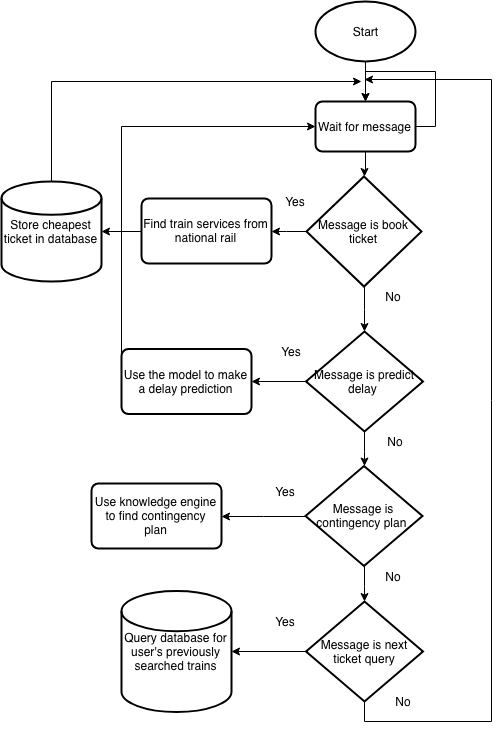
\includegraphics[scale=0.7]{Images/server_flowchart.png}
        \caption{A Flowchart showing how the server should operate.}
        \label{fig:server_flowchat}
    \end{figure}
    
    \section{Implementation}
    
    To create this chatbot, a number of tools and frameworks are required. This project is Python based. Currently, many of the state of the art machine learning tools such as Keras, TensorFlow, Theano, PyTorch and SciKit-Learn are primarily Python based. Therefore, to enable the use of those tools and to allow for the ability to swap and change these tools, one must also use Python. Python also has a lot of support available and a large number of frameworks allowing it to be used for everything this project requires such as server logic.
    
    \subsection{Tools}
    \subsubsection{Facebook Messenger}
    It was decided that to bring the chatbot to the largest amount of users, Facebook's Messenger platform should be used as the chatbot's interface. Using Facebook's this platform would allow users to not only access the chatbot, but to do so without having to install or sign up to a new service. This is important to the project as the goal is not to give users a new platform, but rather to provide a service. It seems that many companies are also doing the same, with over 100,000 active chatbots currently on messenger, most of which are business related \citep{Parr17}. Facebook also gives a unique ID for each user which can be used for identification in the chatbot's database. \\
    
    Following the scandals that Facebook went through recently, their security measures for developers have increased. Applications have to be 'approved' and pass Facebook's security checks before they can be made public. These changes were made to prevent potentially unethical attainment of peoples private information such as gender, hometown etc \citep{Perez18}. This led to some initial difficulty in the chatbot being implemented. It was first, attempted without using the 'Facebook Developers' platform. This led to the page being deleted. However once the chatbot was implemented through the proper avenues, no problems were experienced. In fact by using the developers platform a lot of useful information could be accessed, such as usage statistics, and live API status updates.
    
    \subsection{Frameworks}
    
    \subsubsection{DialogFlow}
    DialogFlow provides the natural language processing (NLP) and natural language generation (NLG) for the chatbot. It integrates with Python through a library, and therefore gives easy access and allows integration with the rest of the project. The reasons behind choosing DialogFlow as an NLP tool over other services such as wit.ai included DialogFlow's capability for dealing with 'small talk', and the ability to create follow up intents that improved the flow of conversation. The documentation provided by Google relating to conversation design also helped greatly in the creation of the chatbot, providing advice on how to 'lead' a user to respond in predictable ways, so that your chatbot rarely misunderstands a message. \\
    
    The flowchart below (Figure \ref{fig:overall_flowchart}) shows a basic example of how a model conversation works, in this case, when a user tries to book a ticket.
    
    \begin{figure}[H]
        \centering
        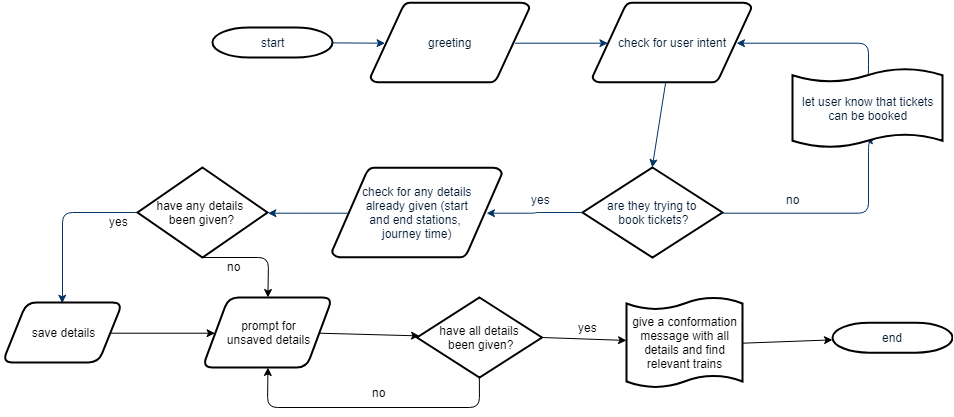
\includegraphics[scale=0.4]{Images/flowchart_overall.png}
        \caption{A flowchart showing the confersational flow when a user tries to book a ticket.}
        \label{fig:overall_flowchart}
    \end{figure}
    
    \subsubsection{PyKnow}
    PyKnow is used as the knowledge engine when dealing with contingency plans for train staff. 
    
    \subsubsection{SciKit-Learn}
    The SciKit-Learn machine learning library provides a number of functions for creating models. It was used to build a model that predicts delay times. Whilst many models were considered, from KNN to an SGD Regressor, eventually it was decided that a random forest should be used. The 'RandomForestRegressor' model from SK-Learn was used as opposed to a standard Random Forest, as predicting delays is a regression task, not a classification one. \\
    
    The reason that an ensemble was selected over any singular classifier is because it has been proven that ensembles regularly attain better performance \citep{Dietterich2000}. This does come at a computing cost, but for relatively small ensembles, this cost is not noticable. The forest model the chatbot employs has 250 trees, which was chosen as a balance. The model gave a good performance at this amount, and increasing the amount of trees increased computing cost for an almost insignificant performance increase. Another reason that the random forest was chosen over a single decision tree is due to the bias-variance tradeoff. A single decision tree can obtain a very low training error, but an unexpectedly high test error due to overfitting. Random Forests counteract this by creating random subsets of features from the dataset, and then building smaller trees from these \citep{Breiman2001}. \\
    
    The dataset that was used to create the model consisted of roughly 200,000 journeys on the Norwich-London Liverpool Street line, and their delays. Unfortunately, the National Rail API has a limit on the amount of information requests you can make, so it was unfeasable to attain enough data for every train line in the UK.
    
    I WILL FINISH THIS ALL LATER THIS EVENING :)
    
    
    \subsubsection{Flask}
    The Flask Python framework was used to build the server logic that handles the recieving and sending of messages. Flask is easy to use and, as it is Python based, integrates well with the rest of the project.
    
    \subsubsection{BeautifulSoup}
    \label{subsubsection:BeautifulSoup}
    BeautifulSoup is a Python HTML parsing library. This will be used for parsing the National Rail website to get information about trains for the user.
    
    \subsubsection{MongoDB \& PyMongo}
    \label{subsubsection:mongodb}
    It was determined that a document based database would be suitable for this project as there appear to be very few relations and the data collected would not benefit from being stored in seperate tables. MongoDB stores data as binary JSON (BSON) \citep{korneliusz_2014} and as such is relatively quick to read and write. These benefits are good to have and contribute to the use of MongoDB and PyMongo over SQL based relational databases.
    
    \subsection{Server}
    \label{subsection:Server}
    Facebook Messenger requires an SSL encrypted connection to send messages to and receive messages from users. This means that a webserver must be set up with an SSL certifacte in order to facilitate this.
    \subsubsection{Microsoft Azure}
    It was decided to use Microsoft's Azure platform as the host for this project. Azure provides Linux VMs and this allows for proper web server configuration and testing.
    
    \subsubsection{NGINX}
    NGINX was used as a reverse proxy to host the Python application. NGINX passes a connection to the Python Flask application and enables easy SSL certificate generation with Let's Encrypt and the Electronic Frontier Foundation's (EFF) Certbot tool %Link to Let's Encrypt and EFF
    
    \subsubsection{Let's Encrypt}
    Let's Encrypt and EFF's Certbot tool was used to generate the SSL certificate for the server. Certbot automatically configures NGINX to use SSL rather than a standard HTTP connection, making the server configuration much easier.
    
    \subsection{Building the System}
    When developing the system a component based approach was used. Each part of the system was developed independently of the overall system and then put together with the server acting as the entry point and the NLP program acts as the overall controller for the rest of the system. Using this method it can be ensured that each component is fully operational before integrating it into the overall system.
    
    \subsection{Server Logic}
    The server recieves a series of HTTP requests from Facebook when a message is sent. The first is a GET request intended to verify that a) Facebook is the platform sending the message and b) Facebook can verify that the server is the one it is expecting. The Second is a POST request containing the user's information (e.g their unique Sender ID) and their message. The message can then be extracted from this POST request and passed to the NLP component. A POST request is then sent on to Facebook containing the NLG response. This response is passed on to the user as a message.
    
    \subsection{Web Scraping}
    There is no publicly available API to get information about sceduled train journeys in the UK. To get around this a web scraping approach had to be used. A number of websites provide train information (e.g. National Rail and Trailine). It was decided to use the National Rail website to gather train information. The first task was to construct the URL that points to a dynamically generated web page containing the train information. This URL is of the format
    \emph{http://ojp.nationalrail.co.uk/service/timesandfares/FROM/TO/DATE/TIME/dep} where \emph{TO} and \emph{FROM} are the 3 letter station codes (e.g NRW for Norwich), \emph{DATE} is the date formatted as \emph{YYMMDD} (year, month and day concatenated) and \emph{TIME} is the intended travel time formatted as \emph{hhmm} (hour and minute concatenated).
    As stated in \ref{subsubsection:BeautifulSoup} the BeautifulSoup library was used to parse the National Rail website and extract the necessary information such as the train time, date and fare. The trains found on the National Rail website are sorted so that the cheapest one is found first and displayed to the user. Functionality was also built to sort the trains in order of their time of departure however the current version has not made such functionality available to the user.
    
    \subsection{Database}
    
    
    \section{Testing}
    \section{Evaluation}
    \section{Discussion}
    
    \bibliographystyle{agsm}
    \bibliography{main.bib}
    
\end{document}